\section{二次曲面}

\begin{problem}{旋转曲面的判定与生成}{Surfaces-Of-Revolution}
    指出下列方程中哪些是旋转曲面，它们是怎样产生的.
    \begin{enumerate}
        \item $\frac{x^{2}}{4}+\frac{y^{2}}{9}+\frac{z^{2}}{9}=1$;
        \item $x^{2}+y^{2}+z^{2}=1$;
        \item $x^{2}+2 y^{2}+34 z^{2}=1$;
        \item $x^{2}-\frac{y^{2}}{4}+z^{2}=1$;
        \item $\frac{x^{2}}{9}+\frac{y^{2}}{16}-\frac{z^{2}}{9}=-1$;
        \item $x^{2}-y^{2}-z^{2}=1$;
        \item $x^{2}+y^{2}=4 z$;
        \item $\frac{x^{2}}{4}-\frac{y^{2}}{9}=3 z$.
    \end{enumerate}
\end{problem}

\begin{solution}
    \ansitem{1} 是旋转曲面。

    方程可写为 $\frac{x^2}{4} + \frac{1}{9}(y^2 + z^2) = 1$。由于 $y^2$ 与 $z^2$ 的系数相同，该曲面可由 $xy$ 平面上的椭圆绕 $x$ 轴旋转而成：
    \begin{equation}
        C: \begin{cases} \frac{x^2}{4} + \frac{y^2}{9} = 1 \\ z = 0 \end{cases} \implies \text{绕 } x \text{ 轴旋转}
    \end{equation}
    \begin{equation}
        \boxed{\text{绕 } x \text{ 轴旋转生成的旋转椭球面}}
    \end{equation}

    \ansitem{2} 是旋转曲面。

    方程中 $x^2, y^2, z^2$ 的系数相等，表示球面。它可以看作由任一坐标平面上的大圆绕其对称轴旋转而成。以绕 $z$ 轴旋转为例：
    \begin{equation}
        C: \begin{cases} x^2 + z^2 = 1 \\ y = 0 \end{cases} \implies \text{绕 } z \text{ 轴旋转}
    \end{equation}
    \begin{equation}
        \boxed{\text{绕 } z \text{ 轴旋转生成的球面}}
    \end{equation}

    \ansitem{3} 不是旋转曲面。

    由于 $x^2, y^2, z^2$ 的系数 $1, 2, 34$ 两两不等，不存在旋转对称性。
    \begin{equation}
        \boxed{\text{该方程不是旋转曲面}}
    \end{equation}

    \ansitem{4} 是旋转曲面。

    方程可写为 $(x^2 + z^2) - \frac{y^2}{4} = 1$。由于 $x^2$ 与 $z^2$ 的系数相同，该曲面可由 $xy$ 平面上的双曲线绕 $y$ 轴旋转而成：
    \begin{equation}
        C: \begin{cases} x^2 - \frac{y^2}{4} = 1 \\ z = 0 \end{cases} \implies \text{绕 } y \text{ 轴旋转}
    \end{equation}
    \begin{equation}
        \boxed{\text{绕 } y \text{ 轴旋转生成的单叶旋转双曲面}}
    \end{equation}

    \ansitem{5} 不是旋转曲面。

    方程中 $x^2, y^2, z^2$ 的系数分别为 $\frac{1}{9}, \frac{1}{16}, -\frac{1}{9}$。不存在两个相同符号且数值相等的系数。
    \begin{equation}
        \boxed{\text{该方程不是旋转曲面}}
    \end{equation}

    \ansitem{6} 是旋转曲面。

    方程可写为 $x^2 - (y^2 + z^2) = 1$。由于 $y^2$ 与 $z^2$ 的系数相同，该曲面可由 $xy$ 平面上的双曲线绕 $x$ 轴旋转而成：
    \begin{equation}
        C: \begin{cases} x^2 - y^2 = 1 \\ z = 0 \end{cases} \implies \text{绕 } x \text{ 轴旋转}
    \end{equation}
    \begin{equation}
        \boxed{\text{绕 } x \text{ 轴旋转生成的双叶旋转双曲面}}
    \end{equation}

    \ansitem{7} 是旋转曲面。

    方程中 $x^2$ 与 $y^2$ 的系数均为 $1$，该曲面可由 $xz$ 平面上的抛物线绕 $z$ 轴旋转而成：
    \begin{equation}
        C: \begin{cases} x^2 = 4z \\ y = 0 \end{cases} \implies \text{绕 } z \text{ 轴旋转}
    \end{equation}
    \begin{equation}
        \boxed{\text{绕 } z \text{ 轴旋转生成的旋转抛物面}}
    \end{equation}

    \ansitem{8} 不是旋转曲面。

    方程中 $x^2$ 与 $y^2$ 的系数互为异号且绝对值不等，该曲面为双曲抛物面（马鞍面）。
    \begin{equation}
        \boxed{\text{该方程不是旋转曲面}}
    \end{equation}
\end{solution}


\begin{problem}{解析几何图形辨析}{Space-Analytic-Geometry}
    指出下列方程在平面直角坐标系 $Oxy$ 和空间直角坐标系 $Oxyz$ 中分别表示怎样的几何图形.
    \begin{enumerate}
        \item $x = 2$;
        \item $y = x + 1$;
        \item $x^2 + y^2 = 4$;
        \item $x^2 - y^2 = 1$;
        \item $y = x^2 + 1$;
        \item $\begin{cases} 5x - y + 1 = 0, \\ 2x - y - 3 = 0; \end{cases}$
        \item $\begin{cases} \dfrac{x^2}{4} + \dfrac{y^2}{9} = 1, \\ y = 2; \end{cases}$
        \item $\begin{cases} \dfrac{x^2}{4} - \dfrac{y^2}{9} = 1, \\ x = 4. \end{cases}$
    \end{enumerate}
\end{problem}

\begin{solution}
    \ansitem{1}

    在 $Oxy$ 中，$x=2$ 确定了所有横坐标为 $2$ 的点；在 $Oxyz$ 中，$z$ 可取任意实数 $\symbb{R}$.
    \begin{equation}
        \boxed{Oxy: \text{垂直于 } x \text{ 轴的直线}; \quad Oxyz: \text{垂直于 } x \text{ 轴的平面}}
    \end{equation}

    \ansitem{2}

    方程为一次线性方程.
    \begin{equation}
        \boxed{Oxy: \text{直线}; \quad Oxyz: \text{平行于 } z \text{ 轴的平面}}
    \end{equation}

    \ansitem{3}

    在空间中，缺少变量 $z$ 的二次方程表示母线平行于 $z$ 轴的柱面.
    \begin{equation}
        \boxed{Oxy: \text{圆}; \quad Oxyz: \text{圆柱面}}
    \end{equation}

    \ansitem{4}

    同理可知其在空间中表示柱面.
    \begin{equation}
        \boxed{Oxy: \text{双曲线}; \quad Oxyz: \text{双曲柱面}}
    \end{equation}

    \ansitem{5}

    同理可知其在空间中表示柱面.
    \begin{equation}
        \boxed{Oxy: \text{抛物线}; \quad Oxyz: \text{抛物柱面}}
    \end{equation}

    \ansitem{6}

    联立方程组：
    \begin{equation}
        \begin{cases} 5x - y + 1 = 0 \\ 2x - y - 3 = 0 \end{cases} \implies 3x + 4 = 0 \implies \begin{cases} x = -\dfrac{4}{3} \\ y = -\dfrac{17}{3} \end{cases}
    \end{equation}
    在 $Oxyz$ 中，两不平行平面的交集为直线.
    \begin{equation}
        \boxed{Oxy: \text{点 } \left( -\dfrac{4}{3}, -\dfrac{17}{3} \right); \quad Oxyz: \text{直线}}
    \end{equation}

    \ansitem{7}

    将 $y=2$ 代入第一式：
    \begin{equation}
        \dfrac{x^2}{4} + \dfrac{4}{9} = 1 \implies x^2 = \dfrac{20}{9} \implies x = \pm \dfrac{2\sqrt{5}}{3}
    \end{equation}
    在 $Oxyz$ 中，交集为两个平面 $x = \pm \dfrac{2\sqrt{5}}{3}$ 与 $y=2$ 的交线.
    \begin{equation}
        \boxed{Oxy: \text{两点 } \left( \pm \dfrac{2\sqrt{5}}{3}, 2 \right); \quad Oxyz: \text{两条平行于 } z \text{ 轴的直线}}
    \end{equation}

    \ansitem{8}

    将 $x=4$ 代入第一式：
    \begin{equation}
        \dfrac{16}{4} - \dfrac{y^2}{9} = 1 \implies \dfrac{y^2}{9} = 3 \implies y = \pm 3\sqrt{3}
    \end{equation}
    \begin{equation}
        \boxed{Oxy: \text{两点 } (4, \pm 3\sqrt{3}); \quad Oxyz: \text{两条平行于 } z \text{ 轴的直线}}
    \end{equation}
\end{solution}


\begin{problem}{旋转曲面}{Surface-of-Revolution}
    求下列旋转曲面的方程，并指出它们的名称.
    \begin{enumerate}
        \item 曲线 $\begin{cases} y^2 - \frac{z^2}{4} = 1, \\ x = 0 \end{cases}$ 绕 $z$ 轴旋转一周;
        \item 曲线 $\begin{cases} y = \sin x \, (0 \le x \le \uppi), \\ z = 0 \end{cases}$ 绕 $x$ 轴旋转一周;
        \item 曲线 $\begin{cases} 4x^2 + 9y^2 = 36, \\ z = 0 \end{cases}$ 绕 $y$ 轴旋转一周.
    \end{enumerate}
\end{problem}

\begin{solution}
    \ansitem{1}

    曲线在 $yOz$ 面上，绕 $z$ 轴旋转，将 $y$ 替换为 $\pm \sqrt{x^2 + y^2}$ 可得曲面方程为
    \begin{equation}
        (\pm \sqrt{x^2 + y^2})^2 - \frac{z^2}{4} = 1 \implies x^2 + y^2 - \frac{z^2}{4} = 1
    \end{equation}
    该曲面为单叶旋转双曲面.
    \begin{equation}
        \boxed{x^2 + y^2 - \frac{z^2}{4} = 1, \quad \text{单叶旋转双曲面}}
    \end{equation}

    \ansitem{2}

    曲线在 $xOy$ 面上，绕 $x$ 轴旋转，将 $y$ 替换为 $\pm \sqrt{y^2 + z^2}$ 可得曲面方程为
    \begin{equation}
        \pm \sqrt{y^2 + z^2} = \sin x \implies y^2 + z^2 = \sin^2 x, \quad 0 \le x \le \uppi
    \end{equation}
    该曲面为旋转曲面.
    \begin{equation}
        \boxed{y^2 + z^2 = \sin^2 x \, (0 \le x \le \uppi), \quad \text{旋转曲面}}
    \end{equation}

    \begin{note}{}{}
        第 (2) 问似乎可以叫「灯笼面」（？）\emoji{grinning-face-with-sweat}
    \end{note}

    \ansitem{3}

    曲线方程变形为 $\frac{x^2}{9} + \frac{y^2}{4} = 1 \, (z=0)$. 绕 $y$ 轴旋转，将 $x$ 替换为 $\pm \sqrt{x^2 + z^2}$ 得
    \begin{equation}
        \frac{(\pm \sqrt{x^2 + z^2})^2}{9} + \frac{y^2}{4} = 1 \implies \frac{x^2 + z^2}{9} + \frac{y^2}{4} = 1
    \end{equation}
    该曲面为旋转椭球面.
    \begin{equation}
        \boxed{\frac{x^2 + z^2}{9} + \frac{y^2}{4} = 1, \quad \text{旋转椭球面}}
    \end{equation}
\end{solution}


\begin{problem}{旋转曲面}{Surface-Of-Revolution}
    求 $Oyz$ 平面上的直线 $y - 2z + 1 = 0$ 绕 $Oyz$ 平面上的直线 $y = z$ 旋转所得旋转曲面的方程.
\end{problem}

\begin{solution}
    设旋转轴为 $L$，其方程为 $\begin{cases} x = 0 \\ y - z = 0 \end{cases}$，方向向量为 $\symbfit{s} = (0, 1, 1)$。\\
    设母线为 $G$，其方程为 $\begin{cases} x = 0 \\ y - 2z + 1 = 0 \end{cases}$。\\
    设 $P(x, y, z)$ 为旋转曲面上任意一点，则在母线 $G$ 上必存在一点 $M_0(0, y_0, z_0)$，使得 $P$ 与 $M_0$ 到旋转轴 $L$ 的距离相等，且 $P, M_0$ 位于垂直于 $L$ 的同一个平面上。

    由 $M_0$ 在母线 $G$ 上知：
    \begin{equation}
        y_0 - 2z_0 + 1 = 0
    \end{equation}
    由于 $P, M_0$ 在垂直于轴 $L$（方向 $\symbfit{s}$）的同一平面上，有 $\symbfit{s} \cdot \overrightarrow{M_0 P} = 0$：
    \begin{equation}
        (0, 1, 1) \cdot (x - 0, y - y_0, z - z_0) = 0 \implies y + z = y_0 + z_0
    \end{equation}
    联立以上两式解得：
    \begin{equation}
        z_0 = \frac{y + z + 1}{3}, \quad y_0 = \frac{2y + 2z - 1}{3}
    \end{equation}
    又点 $P$ 到轴 $L$ 的距离平方为：
    \begin{equation}
        d^2 = \frac{|\symbfit{s} \times \overrightarrow{OP}|^2}{|\symbfit{s}|^2} = \frac{|(z - y) \symbfit{i} + x \symbfit{j} - x \symbfit{k}|^2}{2} = \frac{2x^2 + (y - z)^2}{2}
    \end{equation}
    点 $M_0$ 到轴 $L$ 的距离平方为：
    \begin{equation}
        d_0^2 = \frac{|\symbfit{s} \times \overrightarrow{OM_0}|^2}{|\symbfit{s}|^2} = \frac{(y_0 - z_0)^2}{2}
    \end{equation}
    令 $d^2 = d_0^2$，得：
    \begin{equation}
        2x^2 + (y - z)^2 = (y_0 - z_0)^2
    \end{equation}
    将 $y_0 - z_0 = \frac{2y + 2z - 1 - (y + z + 1)}{3} = \frac{y + z - 2}{3}$ 代入上式：
    \begin{equation}
        \begin{aligned}
                     & 2x^2 + (y - z)^2 = \left( \frac{y + z - 2}{3} \right)^2    \\
            \implies & 18x^2 + 9(y^2 - 2yz + z^2) = y^2 + z^2 + 4 + 2yz - 4y - 4z \\
            \implies & 18x^2 + 8y^2 - 20yz + 8z^2 + 4y + 4z - 4 = 0
        \end{aligned}
    \end{equation}
    化简可得旋转曲面方程为：
    \begin{equation}
        \boxed{9x^2 + 4y^2 - 10yz + 4z^2 + 2y + 2z - 2 = 0}
    \end{equation}
\end{solution}


\begin{problem}{投影直线与旋转曲面}{Projection-Rotation}
    求直线 $L : \frac{x-1}{1}=\frac{y}{1}=\frac{z-1}{-1}$ 在平面 $\pi : x-y+2z-1=0$ 上的投影直线 $L_0$ 的方程，并求 $L_0$ 绕 $y$ 轴旋转一周所得曲面的方程.
\end{problem}

\begin{solution}
    \ansitem{1}

    设直线 $L$ 的方向向量为 $\symbfit{s} = (1, 1, -1)$，平面 $\pi$ 的法向量为 $\symbfit{n} = (1, -1, 2)$.
    过直线 $L$ 且垂直于平面 $\pi$ 的投影平面 $\pi'$ 的法向量为
    \begin{equation}
        \symbfit{n}' = \symbfit{s} \times \symbfit{n} =
        \begin{vmatrix}
            \symbfit{i} & \symbfit{j} & \symbfit{k} \\
            1           & 1           & -1          \\
            1           & -1          & 2
        \end{vmatrix} = (1, -3, -2)
    \end{equation}
    由于 $L$ 经过点 $M(1, 0, 1)$，故投影平面 $\pi'$ 的方程为
    \begin{equation}
        1(x-1) - 3(y-0) - 2(z-1) = 0 \implies x - 3y - 2z + 1 = 0
    \end{equation}
    投影直线 $L_0$ 为平面 $\pi$ 与 $\pi'$ 的交线，其方程为
    \begin{equation}
        \boxed{L_0 : \begin{cases} x - y + 2z - 1 = 0 \\ x - 3y - 2z + 1 = 0 \end{cases}}
    \end{equation}

    \ansitem{2}

    由 $L_0$ 的方程消去 $z$ 可得 $x = 2y$，消去 $x$ 可得 $z = \frac{1-y}{2}$.
    将 $L_0$ 绕 $y$ 轴旋转，曲面上任一点 $(x, y, z)$ 到 $y$ 轴距离的平方等于 $L_0$ 上对应点到 $y$ 轴距离的平方，即
    \begin{equation}
        x^2 + z^2 = [x(y)]^2 + [z(y)]^2
    \end{equation}
    将 $L_0$ 的表达式代入上式得
    \begin{equation}
        x^2 + z^2 = (2y)^2 + \left( \frac{1-y}{2} \right)^2
    \end{equation}
    整理得
    \begin{equation}
        4x^2 + 4z^2 = 16y^2 + 1 - 2y + y^2 \implies 4x^2 - 17y^2 + 4z^2 + 2y - 1 = 0
    \end{equation}
    故所求旋转曲面的方程为
    \begin{equation}
        \boxed{4x^2 - 17y^2 + 4z^2 + 2y - 1 = 0}
    \end{equation}
\end{solution}


\begin{problem}{空间曲面围成的立体}{Surface-Bounded-Solids}
    画出下列各组曲面所围成的立体图形：
    \begin{enumerate}
        \item $\dfrac{x}{3}+\dfrac{y}{2}+z=1,\ x=0,\ y=0,\ z=0$；
        \item $z=x^2+y^2,\ x=0,\ y=0,\ z=0,\ x+y-1=0$；
        \item $z=\sqrt{x^2+y^2},\ x^2+y^2+z^2=R^2$；
        \item $x^2+y^2=2x,\ z=0,\ z=1$；
        \item $x^2+y^2+z^2=R^2,\ x^2+y^2+(z-R)^2=R^2$。
    \end{enumerate}
\end{problem}

\begin{solution}
    \ansitem{1}

    由截距可得
    \begin{equation}
        y=z=0 \implies x=3,\qquad x=z=0 \implies y=2,\qquad x=y=0 \implies z=1.
    \end{equation}

    故所求区域在第一卦限内，顶点为
    \begin{equation}
        O(0,0,0),\qquad A(3,0,0),\qquad B(0,2,0),\qquad C(0,0,1).
    \end{equation}

    \begin{center}
        \begin{tikzpicture}[scale=1]
            \coordinate (O) at (0,0);
            \coordinate (A) at (3,0);
            \coordinate (B) at (-1.2,-1);
            \coordinate (C) at (0,2.3);

            \draw[-latex] (O)--(3.6,0) node[right] {$x$};
            \draw[-latex] (O)--(-1.8,-1.5) node[left] {$y$};
            \draw[-latex] (O)--(0,2.9) node[left] {$z$};

            \fill (O) circle (1.2pt) node[below right] {$O$};
            \fill (A) circle (1.2pt) node[below] {$A$};
            \fill (B) circle (1.2pt) node[left] {$B$};
            \fill (C) circle (1.2pt) node[left] {$C$};

            \draw (A)--(B)--(C)--cycle;
            \draw (O)--(A);
            \draw (O)--(B);
            \draw (O)--(C);
        \end{tikzpicture}
    \end{center}

    \begin{equation}
        \boxed{\text{所围立体}= \text{第一卦限内顶点为 }O,A,B,C\text{ 的四面体}}
    \end{equation}

    \ansitem{2}

    在 $xOy$ 面上的投影由
    \begin{equation}
        x=0,\qquad y=0,\qquad x+y=1
    \end{equation}
    围成，故底面是直角三角形
    \begin{equation}
        D=\bigl\{(x,y)\bigm| x\ge 0,\ y\ge 0,\ x+y\le 1\bigr\}.
    \end{equation}

    又由
    \begin{equation}
        z=0,\qquad z=x^2+y^2
    \end{equation}
    知立体位于抛物面下方、平面 $z=0$ 上方，即
    \begin{equation}
        0\le z\le x^2+y^2.
    \end{equation}

    \begin{center}
        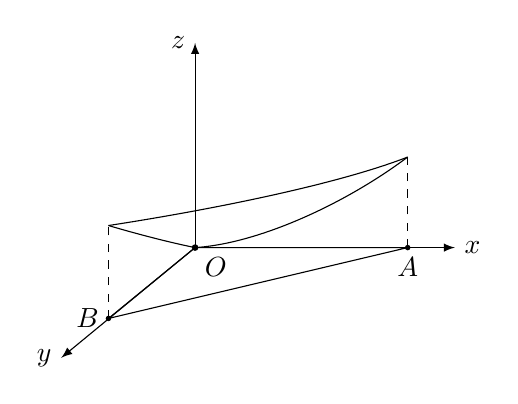
\begin{tikzpicture}[scale=1]
            \coordinate (O) at (0,0);
            \coordinate (A) at (2.7,0);
            \coordinate (B) at (-1.1,-0.9);
            \coordinate (A1) at (2.7,1.15);
            \coordinate (B1) at (-1.1,0.28);

            \draw[-latex] (O)--(3.3,0) node[right] {$x$};
            \draw[-latex] (O)--(-1.7,-1.4) node[left] {$y$};
            \draw[-latex] (O)--(0,2.6) node[left] {$z$};

            \fill (O) circle (1.2pt) node[below right] {$O$};
            \fill (A) circle (1.0pt) node[below] {$A$};
            \fill (B) circle (1.0pt) node[left] {$B$};

            \draw (O)--(A)--(B)--cycle;
            \draw[dashed] (A)--(A1);
            \draw[dashed] (B)--(B1);

            \draw (O) .. controls (0.8,0.05) and (1.9,0.55) .. (A1);
            \draw (O) .. controls (-0.4,0.08) and (-0.9,0.22) .. (B1);
            \draw (A1) .. controls (1.8,0.8) and (0.2,0.48) .. (B1);
        \end{tikzpicture}
    \end{center}

    \begin{equation}
        \boxed{\text{所围立体}= \text{以三角形 }D\text{ 为底、以 }z=x^2+y^2\text{ 为顶的曲顶立体}}
    \end{equation}

    \ansitem{3}

    令
    \begin{equation}
        r=\sqrt{x^2+y^2},
    \end{equation}
    则圆锥面为
    \begin{equation}
        z=r,
    \end{equation}
    球面为
    \begin{equation}
        r^2+z^2=R^2.
    \end{equation}

    联立得交线
    \begin{equation}
        z=r \Longrightarrow 2r^2=R^2 \Longrightarrow r=z=\frac{R}{\sqrt{2}}.
    \end{equation}

    故所求区域为球内且在圆锥 $z=\sqrt{x^2+y^2}$ 内的部分，即
    \begin{equation}
        x^2+y^2+z^2\le R^2,\qquad z\ge \sqrt{x^2+y^2}.
    \end{equation}

    其子午面示意如下：

    \begin{center}
        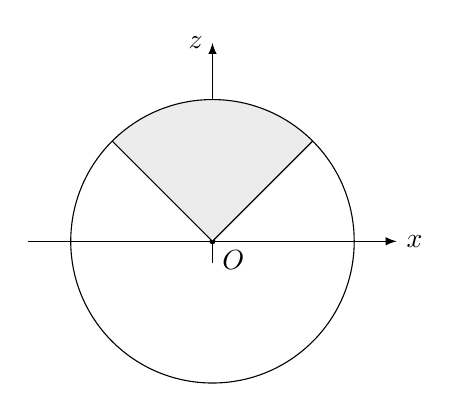
\begin{tikzpicture}[scale=0.9]
            \draw[-latex] (-2.6,0)--(2.6,0) node[right] {$x$};
            \draw[-latex] (0,-0.3)--(0,2.8) node[left] {$z$};

            \fill (0,0) circle (1.2pt) node[below right] {$O$};

            \fill[gray!15] (0,0) -- ({sqrt(2)},{sqrt(2)})
            arc[start angle=45,end angle=135,radius=2] -- cycle;

            \draw (0,0) circle (2);
            \draw ({-sqrt(2)},{sqrt(2)}) -- (0,0) -- ({sqrt(2)},{sqrt(2)});
        \end{tikzpicture}
    \end{center}

    \begin{equation}
        \boxed{\text{所围立体}= \text{球扇形}\bigl(x^2+y^2+z^2\le R^2,\ z\ge \sqrt{x^2+y^2}\bigr)}
    \end{equation}

    \ansitem{4}

    由
    \begin{equation}
        x^2+y^2=2x \Longleftrightarrow (x-1)^2+y^2=1
    \end{equation}
    知侧面为母线平行于 $z$ 轴的圆柱面，其底圆圆心为 $(1,0)$，半径为 $1$。

    再被平面
    \begin{equation}
        z=0,\qquad z=1
    \end{equation}
    截得高为 $1$ 的圆柱体，即
    \begin{equation}
        (x-1)^2+y^2\le 1,\qquad 0\le z\le 1.
    \end{equation}

    \begin{center}
        \begin{tikzpicture}[scale=1]
            \draw[-latex] (0,0)--(3.3,0) node[right] {$x$};
            \draw[-latex] (0,0)--(-1.6,-1.2) node[left] {$y$};
            \draw[-latex] (0,0)--(0,3.0) node[left] {$z$};

            \fill (0,0) circle (1.2pt) node[below right] {$O$};

            \draw (1.0,0) ellipse [x radius=1.0, y radius=0.28];
            \draw (1.0,2.1) ellipse [x radius=1.0, y radius=0.28];
            \draw (0,0)--(0,2.1);
            \draw (2.0,0)--(2.0,2.1);
        \end{tikzpicture}
    \end{center}

    \begin{equation}
        \boxed{\text{所围立体}= \text{轴线平行于 }z\text{ 轴、底圆半径为 }1\text{、高为 }1\text{ 的圆柱体}}
    \end{equation}

    \ansitem{5}

    两球的球心分别为
    \begin{equation}
        O(0,0,0),\qquad O_1(0,0,R).
    \end{equation}

    两球交圈所在平面由两式相减得
    \begin{equation}
        x^2+y^2+z^2=x^2+y^2+(z-R)^2
        \Longrightarrow z=\frac{R}{2}.
    \end{equation}

    交圆半径为
    \begin{equation}
        \rho=\sqrt{R^2-\left(\frac{R}{2}\right)^2}=\frac{\sqrt{3}}{2}R.
    \end{equation}

    故公共部分为两球的重叠区域，即球面透镜。其子午面示意如下：

    \begin{center}
        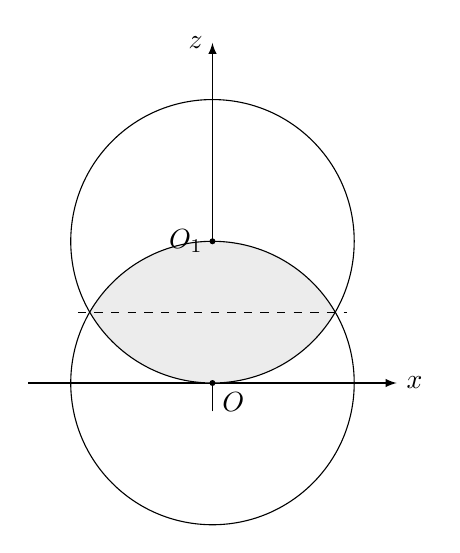
\begin{tikzpicture}[scale=0.9]
            \draw[-latex] (-2.6,0)--(2.6,0) node[right] {$x$};
            \draw[-latex] (0,-0.4)--(0,4.8) node[left] {$z$};

            \begin{scope}
                \clip (0,0) circle (2);
                \fill[gray!15] (0,2) circle (2);
            \end{scope}

            \draw (0,0) circle (2);
            \draw (0,2) circle (2);

            \fill (0,0) circle (1.2pt) node[below right] {$O$};
            \fill (0,2) circle (1.2pt) node[left] {$O_1$};
            \draw[dashed] (-1.9,1)--(1.9,1);
        \end{tikzpicture}
    \end{center}

    \begin{equation}
        \boxed{\text{所围立体}= \text{两等球的公共部分，即球面透镜}}
    \end{equation}
\end{solution}


\begin{problem}{曲面截痕}{Surface-Trace}
    考察曲面 $x^2 - y^2 - z^2 = 9$ 在下列平面上的截痕：
    \begin{enumerate}
        \item $z = 0$;
        \item $x = 0$;
        \item $y = 0$;
        \item $x = 5$.
    \end{enumerate}
\end{problem}

\begin{solution}
    \ansitem{1}
    将 $z = 0$ 代入曲面方程得：
    \begin{equation}
        \begin{cases}
            x^2 - y^2 = 9 \\
            z = 0
        \end{cases}
    \end{equation}
    此截痕在 $xy$ 平面上是双曲线。
    \begin{equation}
        \boxed{\begin{cases} \dfrac{x^2}{9} - \dfrac{y^2}{9} = 1 \\ z = 0 \end{cases}}
    \end{equation}

    \ansitem{2}
    将 $x = 0$ 代入曲面方程得：
    \begin{equation}
        -y^2 - z^2 = 9 \implies y^2 + z^2 = -9
    \end{equation}
    由于在实数范围内 $y^2 + z^2 \ge 0$，方程无实数解。
    \begin{equation}
        \boxed{\text{截痕为空集（无轨迹）}}
    \end{equation}

    \ansitem{3}
    将 $y = 0$ 代入曲面方程得：
    \begin{equation}
        \begin{cases}
            x^2 - z^2 = 9 \\
            y = 0
        \end{cases}
    \end{equation}
    此截痕在 $xz$ 平面上是双曲线。
    \begin{equation}
        \boxed{\begin{cases} \dfrac{x^2}{9} - \dfrac{z^2}{9} = 1 \\ y = 0 \end{cases}}
    \end{equation}

    \ansitem{4}
    将 $x = 5$ 代入曲面方程得：
    \begin{equation}
        25 - y^2 - z^2 = 9 \implies y^2 + z^2 = 16
    \end{equation}
    此截痕在平面 $x = 5$ 上是以 $(5, 0, 0)$ 为圆心，半径为 $4$ 的圆。
    \begin{equation}
        \boxed{\begin{cases} y^2 + z^2 = 16 \\ x = 5 \end{cases}}
    \end{equation}
\end{solution}

\begin{problem}{动点轨迹}{Locus-of-Point}
    一动点 $P(x, y, z)$ 到原点的距离等于它到平面 $z = 4$ 的距离，试求此动点 $P$ 的轨迹，并判定它是什么曲面。
\end{problem}

\begin{solution}
    设动点为 $P(x, y, z)$，根据题意，点 $P$ 到原点 $O(0, 0, 0)$ 的距离为 $\sqrt{x^2 + y^2 + z^2}$，到平面 $z = 4$ 的距离为 $|z - 4|$。由已知条件得：
    \begin{equation}
        \sqrt{x^2 + y^2 + z^2} = |z - 4|
    \end{equation}
    两边平方整理：
    \begin{equation}
        \begin{aligned}
            x^2 + y^2 + z^2          & = (z - 4)^2     \\
            \implies x^2 + y^2 + z^2 & = z^2 - 8z + 16 \\
            \implies x^2 + y^2       & = -8(z - 2)
        \end{aligned}
    \end{equation}
    因此，动点 $P$ 的轨迹方程为：
    \begin{equation}
        \boxed{x^2 + y^2 = -8(z - 2)}
    \end{equation}
    该方程表示一个顶点在 $(0, 0, 2)$，开口向下的旋转抛物面。
\end{solution}


\begin{problem}{柱面方程}{Cylindrical-Surface}
    建立通过两曲面 $x^2 + y^2 + 4z^2 = 1$ 和 $x^2 = y^2 + z^2$ 的交线，而母线平行于 $z$ 轴的柱面方程.
\end{problem}

\begin{solution}
    两曲面的方程联立为
    \begin{equation}
        \begin{cases}
            x^2 + y^2 + 4z^2 = 1 \\
            x^2 = y^2 + z^2
        \end{cases}
    \end{equation}
    由于柱面的母线平行于 $z$ 轴，需在方程组中消去变量 $z$. 由第二个方程可知 $z^2 = x^2 - y^2$, 将其代入第一个方程得
    \begin{equation}
        x^2 + y^2 + 4(x^2 - y^2) = 1 \implies 5x^2 - 3y^2 = 1
    \end{equation}
    故所求柱面方程为
    \begin{equation}
        \boxed{5x^2 - 3y^2 = 1}
    \end{equation}
\end{solution}


\begin{problem}{球面方程}{Sphere-Equation}
    已知一球面经过点 $(0, -3, 1)$ 且与 $Oxy$ 平面交成圆周 $\begin{cases} x^2 + y^2 = 16 \\ z = 0 \end{cases}$，试求其方程.
\end{problem}

\begin{solution}
    设所求球面方程为 $x^2 + y^2 + z^2 + Dx + Ey + Fz + G = 0$. 令 $z = 0$，得其与 $Oxy$ 平面的交线方程为
    \begin{equation}
        \begin{cases}
            x^2 + y^2 + Dx + Ey + G = 0 \\
            z = 0
        \end{cases}
    \end{equation}
    与已知圆周方程对照系数得
    \begin{equation}
        D = 0, \quad E = 0, \quad G = -16
    \end{equation}
    此时球面方程为 $x^2 + y^2 + z^2 + Fz - 16 = 0$. 将点 $(0, -3, 1)$ 代入方程得
    \begin{equation}
        0^2 + (-3)^2 + 1^2 + F \cdot 1 - 16 = 0 \implies F - 6 = 0 \implies F = 6
    \end{equation}
    从而得到该球面的方程为
    \begin{equation}
        \boxed{x^2 + y^2 + z^2 + 6z - 16 = 0}
    \end{equation}
\end{solution}


\begin{problem}{空间曲线在坐标面上的投影}{Curve-Projection}
    建立单叶双曲面 $\frac{x^2}{16} + \frac{y^2}{4} - \frac{z^2}{5} = 1$ 与平面 $x - 2z + 3 = 0$ 的交线在 $Oxy$ 平面上的投影的曲线方程。
\end{problem}

\begin{solution}
    由平面方程 $x - 2z + 3 = 0$ 可解得 $z = \frac{x+3}{2}$，将其代入单叶双曲面方程以消去变量 $z$：
    \begin{equation}
        \frac{x^2}{16} + \frac{y^2}{4} - \frac{1}{5} \left( \frac{x+3}{2} \right)^2 = 1
    \end{equation}
    对上式进行化简推导：
    \begin{equation}
        \begin{aligned}
                                                      & \frac{x^2}{16} + \frac{y^2}{4} - \frac{(x+3)^2}{20} = 1 \\
            \Longrightarrow{\text{等号两边同乘以 } 80} \quad & 5x^2 + 20y^2 - 4(x^2 + 6x + 9) = 80                     \\
            \implies                                  & 5x^2 + 20y^2 - 4x^2 - 24x - 36 = 80                     \\
            \implies                                  & x^2 - 24x + 20y^2 = 116                                 \\
            \Longrightarrow{\text{配方}} \quad          & (x^2 - 24x + 144) + 20y^2 = 116 + 144                   \\
            \implies                                  & (x-12)^2 + 20y^2 = 260
        \end{aligned}
    \end{equation}
    整理得投影柱面方程为 $\frac{(x-12)^2}{260} + \frac{y^2}{13} = 1$。故该交线在 $Oxy$ 平面上的投影曲线方程为：
    \begin{equation}
        \boxed{\begin{cases} \frac{(x-12)^2}{260} + \frac{y^2}{13} = 1 \\ z = 0 \end{cases}}
    \end{equation}
\end{solution}


\begin{problem}{二次曲线与曲面性质研究}{Quadric-Surfaces}
    问在 $Oxy$ 平面中方程 $xy = h$ ($h$ 是或正，或负，或为零的常数) 表示怎样的曲线？在空间坐标系中方程 $xy = z$ 表示什么曲面？试用截口法研究它的图形。
\end{problem}

\begin{solution}
    \ansitem{1}

    在 $Oxy$ 平面中，方程 $xy = h$ 的几何意义取决于 $h$ 的取值：
    当 $h \neq 0$ 时，方程表示以坐标轴为渐近线的等轴双曲线（若 $h > 0$，曲线位于第一、三象限；若 $h < 0$，曲线位于第二、四象限）；
    当 $h = 0$ 时，方程表示两条相交直线，即 $x$ 轴（$y = 0$）与 $y$ 轴（$x = 0$）。

    \ansitem{2}

    在空间坐标系中，方程 $xy = z$ 表示双曲抛物面（俗称马鞍面）。
    利用截口法研究其图形如下：
    \begin{itemize}
        \item \textbf{水平截口}：用平面 $z = k$ 截曲面，得截线为 $\begin{cases} xy = k \\ z = k \end{cases}$。当 $k \neq 0$ 时为等轴双曲线，当 $k$ 由正变负时，双曲线的实轴方向发生 $90^\circ$ 转向；当 $k = 0$ 时为两条交于原点的直线。
        \item \textbf{铅直截口}：用平面 $x = a$ 截之，得直线 $\begin{cases} z = ay \\ x = a \end{cases}$；用平面 $y = b$ 截之，得直线 $\begin{cases} z = bx \\ y = b \end{cases}$。说明该曲面是由两族直线构成的直纹面。
        \item \textbf{对称面截口}：若作坐标旋转 $x = \frac{u+v}{\sqrt{2}}, y = \frac{u-v}{\sqrt{2}}$，方程化为 $z = \frac{u^2}{2} - \frac{v^2}{2}$。用平面 $v = 0$（即 $x-y=0$）截得开口向上的抛物线；用平面 $u = 0$（即 $x+y=0$）截得开口向下的抛物线。
    \end{itemize}
    \begin{equation}
        \boxed{xy = z \text{ 是以原点为鞍点的双曲抛物面}}
    \end{equation}
\end{solution}

\endinput
